\documentclass{article}

\usepackage{amsfonts} 
\usepackage{amsmath} 
\usepackage{graphicx} 
\usepackage{float} 
\usepackage{natbib} 
\usepackage{slashbox} 
\usepackage{graphicx} 
\usepackage{flushend} 
\usepackage{amsmath} 
\usepackage{amssymb} 
\usepackage{amsxtra} 
\usepackage{amstext} 
\usepackage{amsthm} 
\usepackage{amsbsy} 
\usepackage{latexsym} 
\usepackage{mathrsfs} 
\usepackage{eucal} 
\usepackage{synttree} 


\usepackage[spanish]{babel}
\usepackage[utf8x]{inputenc}
\title{Búsqueda con adversarios \\ Inteligencia Artificial}
\author{Flores González Luis Brandon}
\date{24 de Febrero del 2017}


\begin{document}

	\maketitle
	Escribir los pasos de los algoritmos
	
	\begin{enumerate}
		\item Minimax (basta con asignar los valores a los nodos)
			\begin{figure}[H]
				\centering
				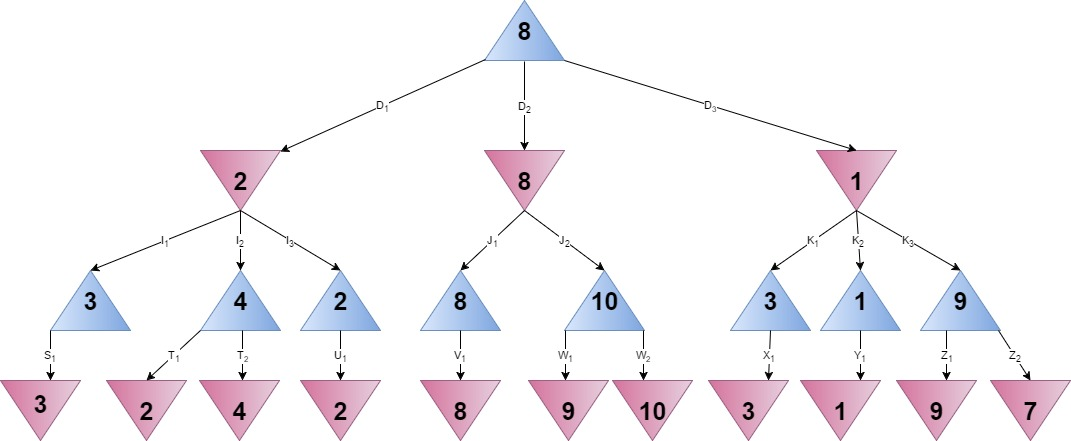
\includegraphics[width=1\textwidth]{imagenes/Minimax}
				\caption{Minimax}
				\label{Minimax}
			\end{figure}
		\item Minimax con poda $\alpha - \beta$ (detallar cómo y en qué orden se van actualizando los valores de $\alpha$ y $\beta$)
		\\\\Se usa recorrido en profundidad, cada imagen corresponde a un paso, cada nodo se ha etiquetado con los valores correspondientes. Además cada rama que no se toma en cuenta esta de color rojo y el resultado final esta de color verde. 
			\begin{figure}[H]
				\centering
				\includegraphics[width=1\textwidth]{imagenes/2}
			\end{figure}
			\begin{figure}[H]
				\centering
				\includegraphics[width=1\textwidth]{imagenes/3}
			\end{figure}
			\begin{figure}[H]
				\centering
				\includegraphics[width=1\textwidth]{imagenes/4}
			\end{figure}
			\begin{figure}[H]
				\centering
				\includegraphics[width=1\textwidth]{imagenes/5}
			\end{figure}
			\begin{figure}[H]
				\centering
				\includegraphics[width=1\textwidth]{imagenes/6}
			\end{figure}
			\begin{figure}[H]
				\centering
				\includegraphics[width=1\textwidth]{imagenes/7}
			\end{figure}
			\begin{figure}[H]
				\centering
				\includegraphics[width=1\textwidth]{imagenes/8}
			\end{figure}
			\begin{figure}[H]
				\centering
				\includegraphics[width=1\textwidth]{imagenes/9}
			\end{figure}
			\begin{figure}[H]
				\centering
				\includegraphics[width=1\textwidth]{imagenes/10}
			\end{figure}
			\begin{figure}[H]
				\centering
				\includegraphics[width=1\textwidth]{imagenes/11}
			\end{figure}
			\begin{figure}[H]
				\centering
				\includegraphics[width=1\textwidth]{imagenes/12}
			\end{figure}
			\begin{figure}[H]
				\centering
				\includegraphics[width=1\textwidth]{imagenes/13}
			\end{figure}	
			\begin{figure}[H]
				\centering
				\includegraphics[width=1\textwidth]{imagenes/14}
			\end{figure}
			\begin{figure}[H]
				\centering
				\includegraphics[width=1\textwidth]{imagenes/15}
			\end{figure}
			\begin{figure}[H]
				\centering
				\includegraphics[width=1\textwidth]{imagenes/16}
			\end{figure}
			\begin{figure}[H]
				\centering
				\includegraphics[width=1\textwidth]{imagenes/17}
			\end{figure}
			\begin{figure}[H]
				\centering
				\includegraphics[width=1\textwidth]{imagenes/18}
			\end{figure}
			\begin{figure}[H]
				\centering
				\includegraphics[width=1\textwidth]{imagenes/19}
			\end{figure}
			\begin{figure}[H]
				\centering
				\includegraphics[width=1\textwidth]{imagenes/20}
			\end{figure}
			\begin{figure}[H]
				\centering
				\includegraphics[width=1\textwidth]{imagenes/21}
			\end{figure}
			\begin{figure}[H]
				\centering
				\includegraphics[width=1\textwidth]{imagenes/22}
			\end{figure}
			\begin{figure}[H]
				\centering
				\includegraphics[width=1\textwidth]{imagenes/23}
			\end{figure}
			\begin{figure}[H]
				\centering
				\includegraphics[width=1\textwidth]{imagenes/24}
			\end{figure}			
			\begin{figure}[H]
				\centering
				\includegraphics[width=1\textwidth]{imagenes/25}
			\end{figure}
	\end{enumerate}
\end{document}